\documentclass[]{standalone}

\usepackage{amsmath}
\usepackage{amsfonts}
\usepackage{amssymb}
\usepackage{graphicx}
\usepackage{tikz}
\usepackage{import}
\usepackage[subpreambles=true]{standalone}

\usepackage{tikz}
\usepackage{tikz-3dplot}

\usetikzlibrary{positioning}

\begin{document}

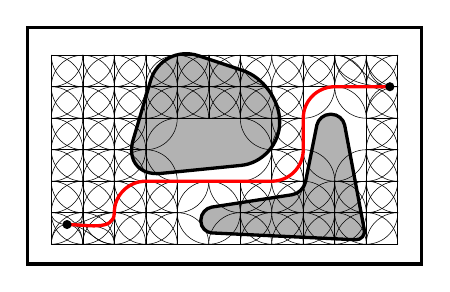
\begin{tikzpicture}[scale=1]
    % \path[draw, fill] (5.5, 3.0) circle (0.05) node[right]{$V_\mathrm{closed}$};
    % \path[draw, fill=gray] (5.5, 2.5) circle (0.05) node[right]{$V_\mathrm{open}$};
    % \path[draw, fill=white] (5.5, 2.0) circle (0.05) node[right]{$V_\mathrm{unvisited}$};

    \useasboundingbox (0,0) rectangle (5,3);

    \coordinate (init) at (0.5,0.5);
    \coordinate (goal) at (4.6,2.25);
    \coordinate (obs1) at (2.4,2.1);
    \coordinate (obs2) at (3.7,0.65);
    \coordinate (seed) at (1.5,1.05);


    \path[draw, very thick, rounded corners=14pt, fill=black!30] (obs1) ++(-1.2,-1) -- ++(2,0.2) -- ++(0,1) -- ++(-1.5,0.5) -- cycle;
    \path[draw, very thick, rounded corners=4pt, fill=black!30] (obs2) ++(-1.5,-0.25) -- ++(0,0.3) -- ++(1.3,0.2) -- ++(0.2,1) -- ++(0.3,0) -- ++(0.3,-1.6) -- cycle;



    \path[draw, very thin] (0.3,2.65) to[in=90,out=0] ++(0.4,-0.4);
    
    \path[draw, very thin] (0.7,2.65) to[in=90,out=0] ++(0.4,-0.4);
    \path[draw, very thin] (0.7,2.65) to ++(-0.4,0);
    \path[draw, very thin] (0.7,2.65) to[in=90,out=180] ++(-0.4,-0.4);
    
    \path[draw, very thin] (1.1,2.65) to[in=90,out=0] ++(0.4,-0.4);
    \path[draw, very thin] (1.1,2.65) to ++(-0.4,0);
    \path[draw, very thin] (1.1,2.65) to[in=90,out=180] ++(-0.4,-0.4);

    \path[draw, very thin] (1.5,2.65) to ++(0.4,0);
    \path[draw, very thin] (1.5,2.65) to[in=90,out=0] ++(0.4,-0.4);
    \path[draw, very thin] (1.5,2.65) to ++(-0.4,0);
    \path[draw, very thin] (1.5,2.65) to[in=90,out=180] ++(-0.4,-0.4);
    
    \path[draw, very thin] (1.9,2.65) to ++(0.4,0);
    \path[draw, very thin] (1.9,2.65) to[in=90,out=0] ++(0.4,-0.4);
    \path[draw, very thin] (1.9,2.65) to[in=90,out=180] ++(-0.4,-0.4);
    
    \path[draw, very thin] (2.3,2.65) to ++(0.4,0);
    \path[draw, very thin] (2.3,2.65) to[in=90,out=0] ++(0.4,-0.4);
    \path[draw, very thin] (2.3,2.65) to[in=90,out=180] ++(-0.4,-0.4);
    
    \path[draw, very thin] (2.7,2.65) to ++(0.4,0);
    \path[draw, very thin] (2.7,2.65) to[in=90,out=0] ++(0.4,-0.4);
    \path[draw, very thin] (2.7,2.65) to[in=90,out=180] ++(-0.4,-0.4);
    
    \path[draw, very thin] (3.1,2.65) to ++(0.4,0);
    \path[draw, very thin] (3.1,2.65) to[in=90,out=0] ++(0.4,-0.4);
    \path[draw, very thin] (3.1,2.65) to[in=90,out=180] ++(-0.4,-0.4);
    
    \path[draw, very thin] (3.5,2.65) to ++(0.4,0);
    \path[draw, very thin] (3.5,2.65) to[in=90,out=0] ++(0.4,-0.4);
    \path[draw, very thin] (3.5,2.65) to[in=90,out=180] ++(-0.4,-0.4);
    
    \path[draw, very thin] (3.9,2.65) to ++(0.4,0);
    \path[draw, very thin] (3.9,2.65) to[in=90,out=0] ++(0.4,-0.4);
    \path[draw, very thin] (3.9,2.65) to[in=90,out=180] ++(-0.4,-0.4);
    
    \path[draw, very thin] (4.3,2.65) to ++(0.4,0);
    \path[draw, very thin] (4.3,2.65) to[in=90,out=0] ++(0.4,-0.4);
    \path[draw, very thin] (4.3,2.65) to[in=90,out=180] ++(-0.4,-0.4);
    
    \path[draw, very thin] (4.7,2.65) to[in=90,out=180] ++(-0.4,-0.4);


    
    \path[draw, very thin] (0.3,2.25) to[in=-90,out=0] ++(0.4,0.4);
    \path[draw, very thin] (0.3,2.25) to[in=90,out=0] ++(0.4,-0.4);
    \path[draw, very thin] (0.3,2.25) to ++(0,-0.4);
    \path[draw, very thin] (0.3,2.25) to ++(0,0.4);
    
    \path[draw, very thin] (0.7,2.25) to[in=-90,out=0] ++(0.4,0.4);
    \path[draw, very thin] (0.7,2.25) to[in=90,out=0] ++(0.4,-0.4);
    \path[draw, very thin] (0.7,2.25) to ++(-0.4,0);
    \path[draw, very thin] (0.7,2.25) to[in=-90,out=180] ++(-0.4,0.4);
    \path[draw, very thin] (0.7,2.25) to[in=90,out=180] ++(-0.4,-0.4);
    \path[draw, very thin] (0.7,2.25) to ++(0,-0.4);
    \path[draw, very thin] (0.7,2.25) to ++(0,0.4);
    
    \path[draw, very thin] (1.1,2.25) to[in=-90,out=0] ++(0.4,0.4);
    \path[draw, very thin] (1.1,2.25) to[in=90,out=0] ++(0.4,-0.4);
    \path[draw, very thin] (1.1,2.25) to ++(-0.4,0);
    \path[draw, very thin] (1.1,2.25) to[in=-90,out=180] ++(-0.4,0.4);
    \path[draw, very thin] (1.1,2.25) to[in=90,out=180] ++(-0.4,-0.4);
    \path[draw, very thin] (1.1,2.25) to ++(0,-0.4);
    \path[draw, very thin] (1.1,2.25) to ++(0,0.4);
    
    \path[draw, very thin] (1.5,2.25) to ++(0.4,0);
    \path[draw, very thin] (1.5,2.25) to[in=-90,out=0] ++(0.4,0.4);
    \path[draw, very thin] (1.5,2.25) to[in=90,out=0] ++(0.4,-0.4);
    \path[draw, very thin] (1.5,2.25) to ++(-0.4,0);
    \path[draw, very thin] (1.5,2.25) to[in=-90,out=180] ++(-0.4,0.4);
    \path[draw, very thin] (1.5,2.25) to[in=90,out=180] ++(-0.4,-0.4);
    \path[draw, very thin] (1.5,2.25) to ++(0,-0.4);
    \path[draw, very thin] (1.5,2.25) to ++(0,0.4);
    
    \path[draw, very thin] (1.9,2.25) to ++(0.4,0);
    \path[draw, very thin] (1.9,2.25) to[in=-90,out=0] ++(0.4,0.4);
    \path[draw, very thin] (1.9,2.25) to[in=90,out=0] ++(0.4,-0.4);
    \path[draw, very thin] (1.9,2.25) to[in=-90,out=180] ++(-0.4,0.4);
    \path[draw, very thin] (1.9,2.25) to[in=90,out=180] ++(-0.4,-0.4);
    \path[draw, very thin] (1.9,2.25) to ++(0,-0.4);
    \path[draw, very thin] (1.9,2.25) to ++(0,0.4);
    
    \path[draw, very thin] (2.3,2.25) to ++(0.4,0);
    \path[draw, very thin] (2.3,2.25) to[in=-90,out=0] ++(0.4,0.4);
    \path[draw, very thin] (2.3,2.25) to[in=90,out=0] ++(0.4,-0.4);
    \path[draw, very thin] (2.3,2.25) to[in=-90,out=180] ++(-0.4,0.4);
    \path[draw, very thin] (2.3,2.25) to[in=90,out=180] ++(-0.4,-0.4);
    \path[draw, very thin] (2.3,2.25) to ++(0,-0.4);
    \path[draw, very thin] (2.3,2.25) to ++(0,0.4);
    
    \path[draw, very thin] (2.7,2.25) to ++(0.4,0);
    \path[draw, very thin] (2.7,2.25) to[in=-90,out=0] ++(0.4,0.4);
    \path[draw, very thin] (2.7,2.25) to[in=90,out=0] ++(0.4,-0.4);
    \path[draw, very thin] (2.7,2.25) to[in=-90,out=180] ++(-0.4,0.4);
    \path[draw, very thin] (2.7,2.25) to[in=90,out=180] ++(-0.4,-0.4);
    \path[draw, very thin] (2.7,2.25) to ++(0,-0.4);
    \path[draw, very thin] (2.7,2.25) to ++(0,0.4);
    
    \path[draw, very thin] (3.1,2.25) to ++(0.4,0);
    \path[draw, very thin] (3.1,2.25) to[in=-90,out=0] ++(0.4,0.4);
    \path[draw, very thin] (3.1,2.25) to[in=90,out=0] ++(0.4,-0.4);
    \path[draw, very thin] (3.1,2.25) to[in=-90,out=180] ++(-0.4,0.4);
    \path[draw, very thin] (3.1,2.25) to[in=90,out=180] ++(-0.4,-0.4);
    
    \path[draw, very thin] (3.5,2.25) to ++(0.4,0);
    \path[draw, very thin] (3.5,2.25) to[in=-90,out=0] ++(0.4,0.4);
    \path[draw, very thin] (3.5,2.25) to[in=-90,out=180] ++(-0.4,0.4);
    \path[draw, very thin] (3.5,2.25) to[in=90,out=180] ++(-0.4,-0.4);
    \path[draw, very thin] (3.5,2.25) to ++(0,-0.4);
    \path[draw, very thin] (3.5,2.25) to ++(0,0.4);
    
    \path[draw, very thin] (3.9,2.25) to ++(0.4,0);
    \path[draw, very thin] (3.9,2.25) to[in=-90,out=0] ++(0.4,0.4);
    \path[draw, very thin] (3.9,2.25) to[in=90,out=0] ++(0.4,-0.4);
    \path[draw, very thin] (3.9,2.25) to[in=-90,out=180] ++(-0.4,0.4);
    \path[draw, very thin] (3.9,2.25) to[in=90,out=180] ++(-0.4,-0.4);
    \path[draw, very thin] (3.9,2.25) to ++(0,0.4);
    
    \path[draw, very thin] (4.3,2.25) to ++(0.4,0);
    \path[draw, very thin] (4.3,2.25) to[in=-90,out=0] ++(0.4,0.4);
    \path[draw, very thin] (4.3,2.25) to[in=90,out=0] ++(0.4,-0.4);
    \path[draw, very thin] (4.3,2.25) to[in=-90,out=180] ++(-0.4,0.4);
    \path[draw, very thin] (4.3,2.25) to ++(0,-0.4);
    \path[draw, very thin] (4.3,2.25) to ++(0,0.4);
    
    \path[draw, very thin] (4.7,2.25) to[in=-90,out=180] ++(-0.4,0.4);
    \path[draw, very thin] (4.7,2.25) to[in=90,out=180] ++(-0.4,-0.4);
    \path[draw, very thin] (4.7,2.25) to ++(0,-0.4);
    \path[draw, very thin] (4.7,2.25) to ++(0,0.4);





    
    \path[draw, very thin] (0.3,1.85) to[in=-90,out=0] ++(0.4,0.4);
    \path[draw, very thin] (0.3,1.85) to[in=90,out=0] ++(0.4,-0.4);
    
    \path[draw, very thin] (0.7,1.85) to[in=-90,out=0] ++(0.4,0.4);
    \path[draw, very thin] (0.7,1.85) to[in=90,out=0] ++(0.4,-0.4);
    \path[draw, very thin] (0.7,1.85) to ++(-0.4,0);
    \path[draw, very thin] (0.7,1.85) to[in=-90,out=180] ++(-0.4,0.4);
    \path[draw, very thin] (0.7,1.85) to[in=90,out=180] ++(-0.4,-0.4);
    
    \path[draw, very thin] (1.1,1.85) to[in=-90,out=0] ++(0.4,0.4);
    \path[draw, very thin] (1.1,1.85) to[in=90,out=0] ++(0.4,-0.4);
    \path[draw, very thin] (1.1,1.85) to ++(-0.4,0);
    \path[draw, very thin] (1.1,1.85) to[in=-90,out=180] ++(-0.4,0.4);
    \path[draw, very thin] (1.1,1.85) to[in=90,out=180] ++(-0.4,-0.4);

    \path[draw, very thin] (1.5,1.85) to ++(0.4,0);
    \path[draw, very thin] (1.5,1.85) to[in=-90,out=0] ++(0.4,0.4);
    \path[draw, very thin] (1.5,1.85) to ++(-0.4,0);
    \path[draw, very thin] (1.5,1.85) to[in=-90,out=180] ++(-0.4,0.4);
    \path[draw, very thin] (1.5,1.85) to[in=90,out=180] ++(-0.4,-0.4);
    
    \path[draw, very thin] (1.9,1.85) to ++(0.4,0);
    \path[draw, very thin] (1.9,1.85) to[in=-90,out=0] ++(0.4,0.4);
    \path[draw, very thin] (1.9,1.85) to[in=-90,out=180] ++(-0.4,0.4);
    \path[draw, very thin] (1.9,1.85) to[in=90,out=180] ++(-0.4,-0.4);
    
    \path[draw, very thin] (2.3,1.85) to ++(0.4,0);
    \path[draw, very thin] (2.3,1.85) to[in=-90,out=0] ++(0.4,0.4);
    \path[draw, very thin] (2.3,1.85) to[in=-90,out=180] ++(-0.4,0.4);
    
    \path[draw, very thin] (2.7,1.85) to ++(0.4,0);
    \path[draw, very thin] (2.7,1.85) to[in=-90,out=0] ++(0.4,0.4);
    \path[draw, very thin] (2.7,1.85) to[in=90,out=0] ++(0.4,-0.4);
    \path[draw, very thin] (2.7,1.85) to[in=-90,out=180] ++(-0.4,0.4);
    
    \path[draw, very thin] (3.1,1.85) to ++(0.4,0);
    \path[draw, very thin] (3.1,1.85) to[in=-90,out=0] ++(0.4,0.4);
    \path[draw, very thin] (3.1,1.85) to[in=90,out=0] ++(0.4,-0.4);
    \path[draw, very thin] (3.1,1.85) to[in=-90,out=180] ++(-0.4,0.4);
    
    \path[draw, very thin] (3.5,1.85) to[in=-90,out=0] ++(0.4,0.4);
    \path[draw, very thin] (3.5,1.85) to[in=-90,out=180] ++(-0.4,0.4);
    \path[draw, very thin] (3.5,1.85) to[in=90,out=180] ++(-0.4,-0.4);
    
    \path[draw, very thin] (4.3,1.85) to ++(0.4,0);
    \path[draw, very thin] (4.3,1.85) to[in=-90,out=0] ++(0.4,0.4);
    \path[draw, very thin] (4.3,1.85) to[in=90,out=0] ++(0.4,-0.4);
    \path[draw, very thin] (4.3,1.85) to[in=-90,out=180] ++(-0.4,0.4);
    
    \path[draw, very thin] (4.7,1.85) to[in=-90,out=180] ++(-0.4,0.4);
    \path[draw, very thin] (4.7,1.85) to[in=90,out=180] ++(-0.4,-0.4);






    \path[draw, very thin] (0.3,1.45) to[in=-90,out=0] ++(0.4,0.4);
    \path[draw, very thin] (0.3,1.45) to[in=90,out=0] ++(0.4,-0.4);
    \path[draw, very thin] (0.3,1.45) to ++(0,-0.4);
    \path[draw, very thin] (0.3,1.45) to ++(0,0.4);
    
    \path[draw, very thin] (0.7,1.45) to[in=-90,out=0] ++(0.4,0.4);
    \path[draw, very thin] (0.7,1.45) to[in=90,out=0] ++(0.4,-0.4);
    \path[draw, very thin] (0.7,1.45) to ++(-0.4,0);
    \path[draw, very thin] (0.7,1.45) to[in=-90,out=180] ++(-0.4,0.4);
    \path[draw, very thin] (0.7,1.45) to[in=90,out=180] ++(-0.4,-0.4);
    \path[draw, very thin] (0.7,1.45) to ++(0,-0.4);
    \path[draw, very thin] (0.7,1.45) to ++(0,0.4);
    
    \path[draw, very thin] (1.1,1.45) to[in=-90,out=0] ++(0.4,0.4);
    \path[draw, very thin] (1.1,1.45) to[in=90,out=0] ++(0.4,-0.4);
    \path[draw, very thin] (1.1,1.45) to ++(-0.4,0);
    \path[draw, very thin] (1.1,1.45) to[in=-90,out=180] ++(-0.4,0.4);
    \path[draw, very thin] (1.1,1.45) to[in=90,out=180] ++(-0.4,-0.4);
    \path[draw, very thin] (1.1,1.45) to ++(0,-0.4);
    \path[draw, very thin] (1.1,1.45) to ++(0,0.4);
    
    \path[draw, very thin] (1.5,1.45) to[in=-90,out=0] ++(0.4,0.4);
    \path[draw, very thin] (1.5,1.45) to[in=90,out=0] ++(0.4,-0.4);
    \path[draw, very thin] (1.5,1.45) to ++(-0.4,0);
    \path[draw, very thin] (1.5,1.45) to[in=-90,out=180] ++(-0.4,0.4);
    \path[draw, very thin] (1.5,1.45) to[in=90,out=180] ++(-0.4,-0.4);
    \path[draw, very thin] (1.5,1.45) to ++(0,-0.4);
    \path[draw, very thin] (1.5,1.45) to ++(0,0.4);
    
    
    \path[draw, very thin] (3.1,1.45) to ++(0.4,0);
    \path[draw, very thin] (3.1,1.45) to[in=-90,out=0] ++(0.4,0.4);
    \path[draw, very thin] (3.1,1.45) to[in=90,out=0] ++(0.4,-0.4);
    \path[draw, very thin] (3.1,1.45) to ++(0,0.4);
    \path[draw, very thin] (3.1,1.45) to ++(0,-0.4);
    \path[draw, very thin] (3.1,1.45) to[in=-90,out=180] ++(-0.4,0.4);
    
    \path[draw, very thin] (3.5,1.45) to[in=90,out=0] ++(0.4,-0.4);
    \path[draw, very thin] (3.5,1.45) to[in=-90,out=180] ++(-0.4,0.4);
    \path[draw, very thin] (3.5,1.45) to[in=90,out=180] ++(-0.4,-0.4);
    \path[draw, very thin] (3.5,1.45) to ++(0,-0.4);
    \path[draw, very thin] (3.5,1.45) to ++(0,0.4);
    
    \path[draw, very thin] (4.3,1.45) to ++(0.4,0);
    \path[draw, very thin] (4.3,1.45) to[in=-90,out=0] ++(0.4,0.4);
    \path[draw, very thin] (4.3,1.45) to[in=90,out=0] ++(0.4,-0.4);
    \path[draw, very thin] (4.3,1.45) to[in=90,out=180] ++(-0.4,-0.4);
    \path[draw, very thin] (4.3,1.45) to ++(0,-0.4);
    \path[draw, very thin] (4.3,1.45) to ++(0,0.4);
    
    \path[draw, very thin] (4.7,1.45) to[in=-90,out=180] ++(-0.4,0.4);
    \path[draw, very thin] (4.7,1.45) to[in=90,out=180] ++(-0.4,-0.4);
    \path[draw, very thin] (4.7,1.45) to ++(0,-0.4);
    \path[draw, very thin] (4.7,1.45) to ++(0,0.4);
    


    
    \path[draw, very thin] (0.3,1.05) to[in=-90,out=0] ++(0.4,0.4);
    \path[draw, very thin] (0.3,1.05) to[in=90,out=0] ++(0.4,-0.4);
    
    \path[draw, very thin] (0.7,1.05) to[in=-90,out=0] ++(0.4,0.4);
    \path[draw, very thin] (0.7,1.05) to[in=90,out=0] ++(0.4,-0.4);
    \path[draw, very thin] (0.7,1.05) to ++(-0.4,0);
    \path[draw, very thin] (0.7,1.05) to[in=-90,out=180] ++(-0.4,0.4);
    \path[draw, very thin] (0.7,1.05) to[in=90,out=180] ++(-0.4,-0.4);
    
    \path[draw, very thin] (1.1,1.05) to[in=-90,out=0] ++(0.4,0.4);
    \path[draw, very thin] (1.1,1.05) to[in=90,out=0] ++(0.4,-0.4);
    \path[draw, very thin] (1.1,1.05) to ++(-0.4,0);
    \path[draw, very thin] (1.1,1.05) to[in=-90,out=180] ++(-0.4,0.4);
    \path[draw, very thin] (1.1,1.05) to[in=90,out=180] ++(-0.4,-0.4);

    \path[draw, very thin] (1.5,1.05) to ++(0.4,0);
    \path[draw, very thin] (1.5,1.05) to[in=90,out=0] ++(0.4,-0.4);
    \path[draw, very thin] (1.5,1.05) to ++(-0.4,0);
    \path[draw, very thin] (1.5,1.05) to[in=-90,out=180] ++(-0.4,0.4);
    \path[draw, very thin] (1.5,1.05) to[in=90,out=180] ++(-0.4,-0.4);
    
    \path[draw, very thin] (1.9,1.05) to ++(0.4,0);
    \path[draw, very thin] (1.9,1.05) to[in=-90,out=180] ++(-0.4,0.4);
    \path[draw, very thin] (1.9,1.05) to[in=90,out=180] ++(-0.4,-0.4);
    
    \path[draw, very thin] (2.3,1.05) to ++(0.4,0);
    \path[draw, very thin] (2.3,1.05) to[in=90,out=0] ++(0.4,-0.4);
    \path[draw, very thin] (2.3,1.05) to[in=90,out=180] ++(-0.4,-0.4);
    
    \path[draw, very thin] (2.7,1.05) to ++(0.4,0);
    \path[draw, very thin] (2.7,1.05) to[in=-90,out=0] ++(0.4,0.4);
    \path[draw, very thin] (2.7,1.05) to[in=90,out=0] ++(0.4,-0.4);
    
    \path[draw, very thin] (3.1,1.05) to ++(0.4,0);
    \path[draw, very thin] (3.1,1.05) to[in=-90,out=0] ++(0.4,0.4);
    \path[draw, very thin] (3.1,1.05) to[in=90,out=0] ++(0.4,-0.4);
    \path[draw, very thin] (3.1,1.05) to[in=90,out=180] ++(-0.4,-0.4);
    
    \path[draw, very thin] (3.5,1.05) to[in=90,out=0] ++(0.4,-0.4);
    \path[draw, very thin] (3.5,1.05) to[in=-90,out=180] ++(-0.4,0.4);
    \path[draw, very thin] (3.5,1.05) to[in=90,out=180] ++(-0.4,-0.4);
    
    \path[draw, very thin] (3.9,1.05) to ++(0.4,0);
    \path[draw, very thin] (3.9,1.05) to[in=-90,out=0] ++(0.4,0.4);
    \path[draw, very thin] (3.9,1.05) to[in=90,out=0] ++(0.4,-0.4);
    \path[draw, very thin] (3.9,1.05) to[in=-90,out=180] ++(-0.4,0.4);
    \path[draw, very thin] (3.9,1.05) to[in=90,out=180] ++(-0.4,-0.4);
    
    \path[draw, very thin] (4.3,1.05) to ++(0.4,0);
    \path[draw, very thin] (4.3,1.05) to[in=-90,out=0] ++(0.4,0.4);
    \path[draw, very thin] (4.3,1.05) to[in=90,out=0] ++(0.4,-0.4);
    \path[draw, very thin] (4.3,1.05) to[in=90,out=180] ++(-0.4,-0.4);
    
    \path[draw, very thin] (4.7,1.05) to[in=-90,out=180] ++(-0.4,0.4);
    \path[draw, very thin] (4.7,1.05) to[in=90,out=180] ++(-0.4,-0.4);
    



    \path[draw, very thin] (0.3,0.65) to[in=-90,out=0] ++(0.4,0.4);
    \path[draw, very thin] (0.3,0.65) to[in=90,out=0] ++(0.4,-0.4);
    \path[draw, very thin] (0.3,0.65) to ++(0,-0.4);
    \path[draw, very thin] (0.3,0.65) to ++(0,0.4);
    
    \path[draw, very thin] (0.7,0.65) to[in=-90,out=0] ++(0.4,0.4);
    \path[draw, very thin] (0.7,0.65) to[in=90,out=0] ++(0.4,-0.4);
    \path[draw, very thin] (0.7,0.65) to ++(-0.4,0);
    \path[draw, very thin] (0.7,0.65) to[in=-90,out=180] ++(-0.4,0.4);
    \path[draw, very thin] (0.7,0.65) to[in=90,out=180] ++(-0.4,-0.4);
    \path[draw, very thin] (0.7,0.65) to ++(0,-0.4);
    \path[draw, very thin] (0.7,0.65) to ++(0,0.4);
    
    \path[draw, very thin] (1.1,0.65) to[in=-90,out=0] ++(0.4,0.4);
    \path[draw, very thin] (1.1,0.65) to[in=90,out=0] ++(0.4,-0.4);
    \path[draw, very thin] (1.1,0.65) to ++(-0.4,0);
    \path[draw, very thin] (1.1,0.65) to[in=-90,out=180] ++(-0.4,0.4);
    \path[draw, very thin] (1.1,0.65) to[in=90,out=180] ++(-0.4,-0.4);
    \path[draw, very thin] (1.1,0.65) to ++(0,-0.4);
    \path[draw, very thin] (1.1,0.65) to ++(0,0.4);
    
    \path[draw, very thin] (1.5,0.65) to ++(0.4,0);
    \path[draw, very thin] (1.5,0.65) to[in=-90,out=0] ++(0.4,0.4);
    \path[draw, very thin] (1.5,0.65) to[in=90,out=0] ++(0.4,-0.4);
    \path[draw, very thin] (1.5,0.65) to ++(-0.4,0);
    \path[draw, very thin] (1.5,0.65) to[in=-90,out=180] ++(-0.4,0.4);
    \path[draw, very thin] (1.5,0.65) to[in=90,out=180] ++(-0.4,-0.4);
    \path[draw, very thin] (1.5,0.65) to ++(0,-0.4);
    \path[draw, very thin] (1.5,0.65) to ++(0,0.4);
    
    \path[draw, very thin] (1.9,0.65) to[in=-90,out=0] ++(0.4,0.4);
    \path[draw, very thin] (1.9,0.65) to[in=90,out=0] ++(0.4,-0.4);
    \path[draw, very thin] (1.9,0.65) to[in=-90,out=180] ++(-0.4,0.4);
    \path[draw, very thin] (1.9,0.65) to[in=90,out=180] ++(-0.4,-0.4);
    \path[draw, very thin] (1.9,0.65) to ++(0,-0.4);
    \path[draw, very thin] (1.9,0.65) to ++(0,0.4);
    
    
    \path[draw, very thin] (2.7,0.65) to ++(0.4,0);
    \path[draw, very thin] (2.7,0.65) to[in=-90,out=0] ++(0.4,0.4);
    \path[draw, very thin] (2.7,0.65) to[in=90,out=0] ++(0.4,-0.4);
    \path[draw, very thin] (2.7,0.65) to[in=-90,out=180] ++(-0.4,0.4);
    \path[draw, very thin] (2.7,0.65) to[in=90,out=180] ++(-0.4,-0.4);
    \path[draw, very thin] (2.7,0.65) to ++(0,-0.4);
    \path[draw, very thin] (2.7,0.65) to ++(0,0.4);
    
    \path[draw, very thin] (3.1,0.65) to ++(0.4,0);
    \path[draw, very thin] (3.1,0.65) to[in=-90,out=0] ++(0.4,0.4);
    \path[draw, very thin] (3.1,0.65) to[in=90,out=0] ++(0.4,-0.4);
    \path[draw, very thin] (3.1,0.65) to[in=-90,out=180] ++(-0.4,0.4);
    \path[draw, very thin] (3.1,0.65) to[in=90,out=180] ++(-0.4,-0.4);
    
    \path[draw, very thin] (3.5,0.65) to ++(0.4,0);
    \path[draw, very thin] (3.5,0.65) to[in=-90,out=0] ++(0.4,0.4);
    \path[draw, very thin] (3.5,0.65) to[in=90,out=0] ++(0.4,-0.4);
    \path[draw, very thin] (3.5,0.65) to[in=-90,out=180] ++(-0.4,0.4);
    \path[draw, very thin] (3.5,0.65) to[in=90,out=180] ++(-0.4,-0.4);
    \path[draw, very thin] (3.5,0.65) to ++(0,-0.4);
    \path[draw, very thin] (3.5,0.65) to ++(0,0.4);
    
    \path[draw, very thin] (3.9,0.65) to ++(0.4,0);
    \path[draw, very thin] (3.9,0.65) to[in=-90,out=0] ++(0.4,0.4);
    \path[draw, very thin] (3.9,0.65) to[in=90,out=0] ++(0.4,-0.4);
    \path[draw, very thin] (3.9,0.65) to[in=-90,out=180] ++(-0.4,0.4);
    \path[draw, very thin] (3.9,0.65) to[in=90,out=180] ++(-0.4,-0.4);
    \path[draw, very thin] (3.9,0.65) to ++(0,-0.4);
    \path[draw, very thin] (3.9,0.65) to ++(0,0.4);
    
    \path[draw, very thin] (4.3,0.65) to ++(0.4,0);
    \path[draw, very thin] (4.3,0.65) to[in=-90,out=0] ++(0.4,0.4);
    \path[draw, very thin] (4.3,0.65) to[in=90,out=0] ++(0.4,-0.4);
    \path[draw, very thin] (4.3,0.65) to[in=-90,out=180] ++(-0.4,0.4);
    \path[draw, very thin] (4.3,0.65) to[in=90,out=180] ++(-0.4,-0.4);
    \path[draw, very thin] (4.3,0.65) to ++(0,-0.4);
    \path[draw, very thin] (4.3,0.65) to ++(0,0.4);
    
    \path[draw, very thin] (4.7,0.65) to[in=-90,out=180] ++(-0.4,0.4);
    \path[draw, very thin] (4.7,0.65) to[in=90,out=180] ++(-0.4,-0.4);
    \path[draw, very thin] (4.7,0.65) to ++(0,-0.4);
    \path[draw, very thin] (4.7,0.65) to ++(0,0.4);
    


    
    \path[draw, very thin] (0.3,0.25) to[in=-90,out=0] ++(0.4,0.4);
    
    \path[draw, very thin] (0.7,0.25) to[in=-90,out=0] ++(0.4,0.4);
    \path[draw, very thin] (0.7,0.25) to ++(-0.4,0);
    \path[draw, very thin] (0.7,0.25) to[in=-90,out=180] ++(-0.4,0.4);
    
    \path[draw, very thin] (1.1,0.25) to[in=-90,out=0] ++(0.4,0.4);
    \path[draw, very thin] (1.1,0.25) to ++(-0.4,0);
    \path[draw, very thin] (1.1,0.25) to[in=-90,out=180] ++(-0.4,0.4);
    
    \path[draw, very thin] (1.5,0.25) to ++(0.4,0);
    \path[draw, very thin] (1.5,0.25) to[in=-90,out=0] ++(0.4,0.4);
    \path[draw, very thin] (1.5,0.25) to ++(-0.4,0);
    \path[draw, very thin] (1.5,0.25) to[in=-90,out=180] ++(-0.4,0.4);
    
    \path[draw, very thin] (1.9,0.25) to ++(0.4,0);
    \path[draw, very thin] (1.9,0.25) to[in=-90,out=180] ++(-0.4,0.4);
    
    \path[draw, very thin] (2.3,0.25) to ++(0.4,0);
    \path[draw, very thin] (2.3,0.25) to[in=-90,out=0] ++(0.4,0.4);
    \path[draw, very thin] (2.3,0.25) to[in=-90,out=180] ++(-0.4,0.4);
    
    \path[draw, very thin] (2.7,0.25) to ++(0.4,0);
    \path[draw, very thin] (2.7,0.25) to[in=-90,out=0] ++(0.4,0.4);
    
    \path[draw, very thin] (3.1,0.25) to ++(0.4,0);
    \path[draw, very thin] (3.1,0.25) to[in=-90,out=0] ++(0.4,0.4);
    \path[draw, very thin] (3.1,0.25) to[in=-90,out=180] ++(-0.4,0.4);
    
    \path[draw, very thin] (3.5,0.25) to ++(0.4,0);
    \path[draw, very thin] (3.5,0.25) to[in=-90,out=0] ++(0.4,0.4);
    \path[draw, very thin] (3.5,0.25) to[in=-90,out=180] ++(-0.4,0.4);
    
    \path[draw, very thin] (3.9,0.25) to ++(0.4,0);
    \path[draw, very thin] (3.9,0.25) to[in=-90,out=0] ++(0.4,0.4);
    \path[draw, very thin] (3.9,0.25) to[in=-90,out=180] ++(-0.4,0.4);
    
    \path[draw, very thin] (4.3,0.25) to ++(0.4,0);
    \path[draw, very thin] (4.3,0.25) to[in=-90,out=0] ++(0.4,0.4);
    \path[draw, very thin] (4.3,0.25) to[in=-90,out=180] ++(-0.4,0.4);
    
    \path[draw, very thin] (init) to[in=-90,out=0] (0.7,0.65);
    \path[draw, very thin] (init) to[in=-90,out=0] (1.1,0.65);
    \path[draw, very thin] (init) to[in=-180,out=0] (1.1,0.65);
    \path[draw, very thin] (init) to[in=90,out=0] (1.1,0.25);
    \path[draw, very thin] (init) to[in=-180,out=0] (1.1,0.25);
    \path[draw, very thin] (init) to[in=90,out=0] (0.7,0.25);
    \path[draw, very thin] (init) to[in=-90,out=180] (0.3,0.65);
    \path[draw, very thin] (init) to[in=90,out=180] (0.3,0.25);
    
    
    \path[draw, very thin] (goal) to[in=0,out=180] (4.3,2.25);
    \path[draw, very thin] (goal) to[in=-90,out=180] (4.3,2.65);
    \path[draw, very thin] (goal) to[in=90,out=180] (4.3,1.85);
    \path[draw, very thin] (goal) to[in=0,out=180] (3.9,2.25);
    \path[draw, very thin] (goal) to[in=-90,out=180] (3.9,2.65);
    \path[draw, very thin] (goal) to[in=0,out=180] (3.9,2.65);
    \path[draw, very thin] (goal) to[in=180,out=0] (4.7,2.25);
    

    \path[draw=red, very thick] (init) to[out=0,in=-90] (1.1,0.65) to[out=90,in=180] ++(0.4,0.4) to ++(0.4,0) to ++(0.4,0) to ++(0.4,0.0) to ++(0.4,0) to[out=0,in=-90] ++(0.4,0.4) to ++(0,0.4) to[out=90,in=180] ++(0.4,0.4) to (goal);
    

    \path[draw, very thick] (0,0) -- (5,0) -- (5,3) -- (0,3) -- cycle;
    
    \path[draw, fill=black] (init) circle (0.05);

    \path[draw, fill=black] (goal) circle (0.05);

    % \path[draw, fill=black] (init) circle (0.05) node[below=1.4mm] {$x_\mathrm{init}$};

    % \path[draw, fill=black] (goal) circle (0.05) node[shift={(0.05,0.25)}] {$x_\mathrm{goal}$};

\end{tikzpicture}
\end{document}